%!TEX root = widefieldscan.tex
\svnidlong
{$HeadURL$}
{$LastChangedDate$}
{$LastChangedRevision$}
{$LastChangedBy$}
%
%\ifhtml
%\else
%\begin{center}
%	\fbox{
%		\begin{minipage}{.618\columnwidth}
%		The section below is versioned at \url{\svnkw{HeadURL}} (last commit @ \svnfileday.\svnfilemonth.\svnfileyear \space \svnfilehour:\svnfileminute, Revision: \svnkw{LastChangedRevision}).
%		\end{minipage}
%	} 
%\end{center}
%\fi
%
\section{Results}\label{sec:Results}%
\subsection{Image Merging and Reconstruction}\label{sec:Image Merging and Reconstruction}%
Multiple independently acquired projection images covering the desired field of view have been merged into single projections covering the full field of view. Figure~\ref{fig:wide field scan results}a) shows corrected projection images from three overlapping subscans prior to merging (with marked overlapping regions). Figure~\ref{fig:wide field scan results}b) shows one merged projection image prior to reconstruction and figure~\ref{fig:wide field scan results}c) shows one slice of the reconstructed dataset of protocol B, acquired from 5244 projections. Such a reconstructed slice covers a field of view of 2792$\times$2792 pixels (4.13$\times$\SI{4.13}{\milli\meter}) which is three times the size of what can be achieved with one single binned scan (1024 pixels or \SI{1.52}{\milli\meter}). %1024 * 1.48 um/px = 1.51552mm

\ifiucr
	\begin{figure}%
			\caption{Wide field scan of a rat lung sample obtained from a Sprague-Dawley rat 21 days after birth, showing the distal-medial edge of the right lower lung lobe. The sample has been scanned at \SI{12.6}{\kilo\electronvolt}, the protocol details conform to protocol B, described in table~\ref{tab:protocols}. %
		a) Three uncorrected and independent projection images from subscans s$_1$--s$_3$, each with a size of 1024\(\times\)1024 pixels at a resolution of \SI{1.48}{\micro\meter\per pixel}, each covering a field of view of \SI{1.52}{\milli\meter}. Subscans s$_1$ and s$_2$ overlap each other by 141 pixels (red and green overlay), subscans s$_2$ and s$_3$ overlap each other by 138 pixels (blue and yellow overlay). 5244 projections over a rotation of \SI{180}{\degree} have been acquired for all subscans. %
		b) Merged and corrected image from the three subscans shown in subfigure a). Each merged projection has a size of 2793\(\times\)1024 pixels at a resolution of \SI{1.48}{\micro\meter\per pixel}. The width of the merged projections is slightly smaller than three times the width of the subscans due to the overlap needed to merge the projections (2793~px$=3072$~px$-141$~px$-138$~px). Since the x-ray beam is extremely stable, the bands visible in the raw projections can be eliminated. %
		c) Cropped slice of the tomographic dataset reconstructed from 5244 merged projections shown in subfigure b). Due to the coherence of the x-ray beam the air-to-paraffin interface is visible around the sample.%
		}%
		\label{fig:wide field scan results}%
		%\documentclass{article}
%\usepackage{subfig}
%\usepackage{tikz}
%\usepackage{siunitx}
%\begin{document}
%\newcommand{\imsize}{\linewidth}
%\newlength\imagewidth % needed for scalebars
%\newlength\imagescale % needed for scalebars
%\begin{figure}
%	\centering
%%%%%%%%%%%%%%%%%%%%%%%%%%%%%
	\renewcommand{\imsize}{.333\linewidth}
	\pgfmathsetlength{\imagewidth}{\imsize} % desired display width of image
	\pgfmathsetlength{\imagescale}{\imagewidth/1024} % pixel width of image
			% --------------------------------------------------------------
			% Cutline between SubScan 1 and 2: 141 pixels
			% Cutline between SubScan 2 and 3: 138 pixels
			% --------------------------------------------------------------
			\def\size{1023}%
			\begin{tikzpicture}[x=\imagescale,y=-\imagescale]%
				\node[anchor=north west,inner sep=0pt,outer sep=0pt] at (0,0)%
					{\includegraphics[width=\imagewidth]{img/merge/R108C21Cb_s13358_normalize}};%
%					{\includegraphics[width=\imagewidth]{R108C21Cb_s13358_normalize}};%
				\def\overlap{141}%
				\fill [red, nearly transparent] (1024-\overlap,1) rectangle (\size,\size);%
				\draw (1024-\overlap,1) rectangle (\size,\size);%
				\node [anchor=center, color=white] at (100,1024-100) {a)};				
			\end{tikzpicture}%
			\begin{tikzpicture}[x=\imagescale,y=-\imagescale]%
				\node[anchor=north west,inner sep=0pt,outer sep=0pt] at (0,0)%
					{\includegraphics[width=\imagewidth]{img/merge/R108C21Cb_s23358_normalize}};%
%					{\includegraphics[width=\imagewidth]{R108C21Cb_s23358_normalize}};%
				\def\overlap{141}%
				\fill [green, nearly transparent] (1,1) rectangle (\overlap,\size);%
				\draw (1,1) rectangle (\overlap,\size);%
				\def\overlap{138}%
				\fill [blue, nearly transparent] (1024-\overlap,1) rectangle (\size,\size);%
				\draw (1024-\overlap,1) rectangle (\size,\size);%
			\end{tikzpicture}%
			\begin{tikzpicture}[x=\imagescale,y=-\imagescale]%
				% place image (integer coordinates refer to pixel centers):
				\node[anchor=north west,inner sep=0pt,outer sep=0pt] at (0,0)%
					{\includegraphics[width=\imagewidth]{img/merge/R108C21Cb_s33358_normalize}};%
%					{\includegraphics[width=\imagewidth]{R108C21Cb_s33358_normalize}};%
				\def\overlap{138}%
				\fill [yellow, nearly transparent] (1,1) rectangle (\overlap,\size);%
				\draw (1,1) rectangle (\overlap,\size);%
				\draw[|-|,thick] (5,200) -- (1021,200) node [color=white,midway,above] {\SI{1.51552}{\milli\meter}};%
				\def\x{924}% 1024 - 100
				\def\y{922}% 1024 * .9 = 921.6
				\def\bar{338}% 100 px = 148 um
				\draw[|-|,thick,color=white] (\x-\bar,\y) -- (\x,\y) node [midway,above] {\SI{500}{\micro\meter}};%
			\end{tikzpicture}%
			\label{fig:subscans}%
%%%%%%%%%%%%%%%%%%%%%%%%%%%%%	
%	\caption{caption}
%\end{figure}
%\end{document}\\%
		%\documentclass{article}
%\usepackage{subfig}
%\usepackage{tikz}
%\usepackage{siunitx}
%\begin{document}
%\newcommand{\imsize}{\linewidth}
%\newlength\imagewidth % needed for scalebars
%\newlength\imagescale % needed for scalebars
%\begin{figure}
%	\centering
%%%%%%%%%%%%%%%%%%%%%%%%%%%%%
		\renewcommand{\imsize}{\linewidth}%
		\pgfmathsetlength{\imagewidth}{\imsize} % desired displayed width of image
		\pgfmathsetlength{\imagescale}{\imagewidth/2793}% pixel width of image
			\begin{tikzpicture}[x=\imagescale,y=-\imagescale]%
				\node[anchor=north west,inner sep=0pt,outer sep=0pt] at (0,0)%
					{\includegraphics[width=\imagewidth]{img/merge/R108C21Cb_mrg3333_normalize}};%
%					{\includegraphics[width=\imagewidth]{R108C21Cb_mrg3333_normalize}};%
				\def\x{2693} % 2793-100
				\def\y{922} % 1024*.9 = 921.6
				\def\bar{338} % 100 px = 148 um
				\draw[|-|,thick,color=white] (5,256) -- (2787,256) node [midway,above] {\SI{4.13364}{\milli\meter}};
				\draw[|-|,thick,color=white] (\x-\bar,\y) -- (\x,\y) node [midway,above] {\SI{500}{\micro\meter}};
				\node [anchor=center, color=white] at (100,1024-100) {b)};
				\end{tikzpicture}%
			\label{fig:merge-proj}%
%%%%%%%%%%%%%%%%%%%%%%%%%%%%%	
%	\caption{caption}
%\end{figure}
%\end{document}\\%
		%\documentclass{article}
%\usepackage{subfig}
%\usepackage{tikz}
%\usepackage{siunitx}
%\begin{document}
%\newcommand{\imsize}{\linewidth}
%\newlength\imagewidth % needed for scalebars
%\newlength\imagescale % needed for scalebars
%\begin{figure}
%	\centering
%%%%%%%%%%%%%%%%%%%%%%%%%%%%%
		\pgfmathsetlength{\imagewidth}{\imsize}%
		\pgfmathsetlength{\imagescale}{\imagewidth/2792}%
			\begin{tikzpicture}[x=\imagescale,y=-\imagescale]%
				\node [anchor=north west,inner sep=0pt,outer sep=0pt] at (0,0)%
					{\includegraphics[width=\imagewidth]{img/merge/R108C21Cb_mrg1024rec8bit}};% ``mogrify -shave 0x900 -format png R108C21Cb_mrg1024rec8bit.tif''
%					{\includegraphics[width=\imagewidth]{R108C21Cb_mrg1024rec8bit}};
				\clip (0,0) rectangle (2792,992);				
				\def\x{2692} % 2792-100
				\def\y{893} % 992 * .9 = 892.8
				\def\bar{338} % 100 px = 148 um
				%%%% scalebar
					\draw[|-|,thick,color=white] (\x-\bar,\y) -- (\x,\y) node [midway, above] {\SI{500}{\micro\meter}};
%					\draw[|-|,thick,color=white] (5,30) -- (2787,30) node [midway, below] {\SI{4.13216}{\milli\meter}};
				%%%% big circle
					\draw [dashed, ultra thick, color=red] (2792/2,992/2) circle (512);
					\def\angle{35}
					\draw [white, thick, <->] (2792/2,992/2) +(\angle:0) --  node (bigto) {} +(\angle:512); 
					\node [white] (bigfrom) at (349,256){$\frac{1024}{2}$px};
					\draw [white, ->, thick, densely dotted] (bigfrom) to [bend left=45] (bigto);
				%%%% big circle
				%%%% 141px circle
				\draw [dashed, ultra thick, color=red] (2792/2,992/2) circle (512-141);
				\def\angle{35+90}
					\draw [white,thick,<->] (2792/2,992/2) +(\angle:0) -- node (smallto) {} +(\angle:512-141);
					\node [white] (smallfrom) at (349,384) {$\frac{1024}{2}-141$px};
					\draw [white, ->, thick, densely dotted] (smallfrom) to [bend left=45] (smallto);
				%%%% 141px circle					
%				%%%% 138px circle
%				\draw [dashed,color=red] (2792/2,992/2) circle (512-138);
%				\def\angle{45+90+90}
%					\draw [white,<->] (2792/2,992/2) +(\angle:0) -- node (vsmallto) {} +(\angle:512-138);
%					\node [white] (vsmallfrom) at (2972-768,992-512) {$\frac{1024}{2}-138$px};
%					\draw [white,->,densely dotted] (vsmallfrom) to [bend right=45] (vsmallto);
%				%%%% 138px circle
				%%%% center
				\fill [color=red] (2792/2,992/2) circle (5);
				%%%% center
				%%%% inset
%				\newcommand{\size}{.2\imagewidth}%
%				\clip (256,256) rectangle (512,512);
%				\node[anchor=north west,inner sep=0pt,outer sep=0pt] at (0,0)
%					{\includegraphics[width=\size]{R108C21Cb_mrg1024rec8bit}};
%					\draw[white] (0,0) rectangle (\size,-\size);
				%%%% inset
				\node [anchor=south west, color=white] at (0,990) {(c)};			
				\end{tikzpicture}%
			\label{fig:merge-rec}%
%%%%%%%%%%%%%%%%%%%%%%%%%%%%%	
%	\caption{caption}
%\end{figure}
%\end{document}\\%
	\end{figure}%
\else
	\begin{figure}[htp]%
		%\documentclass{article}
%\usepackage{subfig}
%\usepackage{tikz}
%\usepackage{siunitx}
%\begin{document}
%\newcommand{\imsize}{\linewidth}
%\newlength\imagewidth % needed for scalebars
%\newlength\imagescale % needed for scalebars
%\begin{figure}
%	\centering
%%%%%%%%%%%%%%%%%%%%%%%%%%%%%
	\renewcommand{\imsize}{.333\linewidth}
	\pgfmathsetlength{\imagewidth}{\imsize} % desired display width of image
	\pgfmathsetlength{\imagescale}{\imagewidth/1024} % pixel width of image
			% --------------------------------------------------------------
			% Cutline between SubScan 1 and 2: 141 pixels
			% Cutline between SubScan 2 and 3: 138 pixels
			% --------------------------------------------------------------
			\def\size{1023}%
			\begin{tikzpicture}[x=\imagescale,y=-\imagescale]%
				\node[anchor=north west,inner sep=0pt,outer sep=0pt] at (0,0)%
					{\includegraphics[width=\imagewidth]{img/merge/R108C21Cb_s13358_normalize}};%
%					{\includegraphics[width=\imagewidth]{R108C21Cb_s13358_normalize}};%
				\def\overlap{141}%
				\fill [red, nearly transparent] (1024-\overlap,1) rectangle (\size,\size);%
				\draw (1024-\overlap,1) rectangle (\size,\size);%
				\node [anchor=center, color=white] at (100,1024-100) {a)};				
			\end{tikzpicture}%
			\begin{tikzpicture}[x=\imagescale,y=-\imagescale]%
				\node[anchor=north west,inner sep=0pt,outer sep=0pt] at (0,0)%
					{\includegraphics[width=\imagewidth]{img/merge/R108C21Cb_s23358_normalize}};%
%					{\includegraphics[width=\imagewidth]{R108C21Cb_s23358_normalize}};%
				\def\overlap{141}%
				\fill [green, nearly transparent] (1,1) rectangle (\overlap,\size);%
				\draw (1,1) rectangle (\overlap,\size);%
				\def\overlap{138}%
				\fill [blue, nearly transparent] (1024-\overlap,1) rectangle (\size,\size);%
				\draw (1024-\overlap,1) rectangle (\size,\size);%
			\end{tikzpicture}%
			\begin{tikzpicture}[x=\imagescale,y=-\imagescale]%
				% place image (integer coordinates refer to pixel centers):
				\node[anchor=north west,inner sep=0pt,outer sep=0pt] at (0,0)%
					{\includegraphics[width=\imagewidth]{img/merge/R108C21Cb_s33358_normalize}};%
%					{\includegraphics[width=\imagewidth]{R108C21Cb_s33358_normalize}};%
				\def\overlap{138}%
				\fill [yellow, nearly transparent] (1,1) rectangle (\overlap,\size);%
				\draw (1,1) rectangle (\overlap,\size);%
				\draw[|-|,thick] (5,200) -- (1021,200) node [color=white,midway,above] {\SI{1.51552}{\milli\meter}};%
				\def\x{924}% 1024 - 100
				\def\y{922}% 1024 * .9 = 921.6
				\def\bar{338}% 100 px = 148 um
				\draw[|-|,thick,color=white] (\x-\bar,\y) -- (\x,\y) node [midway,above] {\SI{500}{\micro\meter}};%
			\end{tikzpicture}%
			\label{fig:subscans}%
%%%%%%%%%%%%%%%%%%%%%%%%%%%%%	
%	\caption{caption}
%\end{figure}
%\end{document}\\%
		%\documentclass{article}
%\usepackage{subfig}
%\usepackage{tikz}
%\usepackage{siunitx}
%\begin{document}
%\newcommand{\imsize}{\linewidth}
%\newlength\imagewidth % needed for scalebars
%\newlength\imagescale % needed for scalebars
%\begin{figure}
%	\centering
%%%%%%%%%%%%%%%%%%%%%%%%%%%%%
		\renewcommand{\imsize}{\linewidth}%
		\pgfmathsetlength{\imagewidth}{\imsize} % desired displayed width of image
		\pgfmathsetlength{\imagescale}{\imagewidth/2793}% pixel width of image
			\begin{tikzpicture}[x=\imagescale,y=-\imagescale]%
				\node[anchor=north west,inner sep=0pt,outer sep=0pt] at (0,0)%
					{\includegraphics[width=\imagewidth]{img/merge/R108C21Cb_mrg3333_normalize}};%
%					{\includegraphics[width=\imagewidth]{R108C21Cb_mrg3333_normalize}};%
				\def\x{2693} % 2793-100
				\def\y{922} % 1024*.9 = 921.6
				\def\bar{338} % 100 px = 148 um
				\draw[|-|,thick,color=white] (5,256) -- (2787,256) node [midway,above] {\SI{4.13364}{\milli\meter}};
				\draw[|-|,thick,color=white] (\x-\bar,\y) -- (\x,\y) node [midway,above] {\SI{500}{\micro\meter}};
				\node [anchor=center, color=white] at (100,1024-100) {b)};
				\end{tikzpicture}%
			\label{fig:merge-proj}%
%%%%%%%%%%%%%%%%%%%%%%%%%%%%%	
%	\caption{caption}
%\end{figure}
%\end{document}\\%
		%\documentclass{article}
%\usepackage{subfig}
%\usepackage{tikz}
%\usepackage{siunitx}
%\begin{document}
%\newcommand{\imsize}{\linewidth}
%\newlength\imagewidth % needed for scalebars
%\newlength\imagescale % needed for scalebars
%\begin{figure}
%	\centering
%%%%%%%%%%%%%%%%%%%%%%%%%%%%%
		\pgfmathsetlength{\imagewidth}{\imsize}%
		\pgfmathsetlength{\imagescale}{\imagewidth/2792}%
			\begin{tikzpicture}[x=\imagescale,y=-\imagescale]%
				\node [anchor=north west,inner sep=0pt,outer sep=0pt] at (0,0)%
					{\includegraphics[width=\imagewidth]{img/merge/R108C21Cb_mrg1024rec8bit}};% ``mogrify -shave 0x900 -format png R108C21Cb_mrg1024rec8bit.tif''
%					{\includegraphics[width=\imagewidth]{R108C21Cb_mrg1024rec8bit}};
				\clip (0,0) rectangle (2792,992);				
				\def\x{2692} % 2792-100
				\def\y{893} % 992 * .9 = 892.8
				\def\bar{338} % 100 px = 148 um
				%%%% scalebar
					\draw[|-|,thick,color=white] (\x-\bar,\y) -- (\x,\y) node [midway, above] {\SI{500}{\micro\meter}};
%					\draw[|-|,thick,color=white] (5,30) -- (2787,30) node [midway, below] {\SI{4.13216}{\milli\meter}};
				%%%% big circle
					\draw [dashed, ultra thick, color=red] (2792/2,992/2) circle (512);
					\def\angle{35}
					\draw [white, thick, <->] (2792/2,992/2) +(\angle:0) --  node (bigto) {} +(\angle:512); 
					\node [white] (bigfrom) at (349,256){$\frac{1024}{2}$px};
					\draw [white, ->, thick, densely dotted] (bigfrom) to [bend left=45] (bigto);
				%%%% big circle
				%%%% 141px circle
				\draw [dashed, ultra thick, color=red] (2792/2,992/2) circle (512-141);
				\def\angle{35+90}
					\draw [white,thick,<->] (2792/2,992/2) +(\angle:0) -- node (smallto) {} +(\angle:512-141);
					\node [white] (smallfrom) at (349,384) {$\frac{1024}{2}-141$px};
					\draw [white, ->, thick, densely dotted] (smallfrom) to [bend left=45] (smallto);
				%%%% 141px circle					
%				%%%% 138px circle
%				\draw [dashed,color=red] (2792/2,992/2) circle (512-138);
%				\def\angle{45+90+90}
%					\draw [white,<->] (2792/2,992/2) +(\angle:0) -- node (vsmallto) {} +(\angle:512-138);
%					\node [white] (vsmallfrom) at (2972-768,992-512) {$\frac{1024}{2}-138$px};
%					\draw [white,->,densely dotted] (vsmallfrom) to [bend right=45] (vsmallto);
%				%%%% 138px circle
				%%%% center
				\fill [color=red] (2792/2,992/2) circle (5);
				%%%% center
				%%%% inset
%				\newcommand{\size}{.2\imagewidth}%
%				\clip (256,256) rectangle (512,512);
%				\node[anchor=north west,inner sep=0pt,outer sep=0pt] at (0,0)
%					{\includegraphics[width=\size]{R108C21Cb_mrg1024rec8bit}};
%					\draw[white] (0,0) rectangle (\size,-\size);
				%%%% inset
				\node [anchor=south west, color=white] at (0,990) {(c)};			
				\end{tikzpicture}%
			\label{fig:merge-rec}%
%%%%%%%%%%%%%%%%%%%%%%%%%%%%%	
%	\caption{caption}
%\end{figure}
%\end{document}%
			\caption{Wide field scan of a rat lung sample obtained from a Sprague-Dawley rat 21 days after birth, showing the distal-medial edge of the right lower lung lobe. The sample has been scanned at \SI{12.6}{\kilo\electronvolt}, the protocol details conform to protocol B, described in table~\ref{tab:protocols}. %
		a) Three uncorrected and independent projection images from subscans s$_1$--s$_3$, each with a size of 1024\(\times\)1024 pixels at a resolution of \SI{1.48}{\micro\meter} per pixel, each covering a field of view of \SI{1.52}{\milli\meter}. Subscans s$_1$ and s$_2$ overlap each other by 141 pixels (red and green overlay), subscans s$_2$ and s$_3$ overlap each other by 138 pixels (blue and yellow overlay). 5244 projections over a rotation of \SI{180}{\degree} have been acquired for all subscans. %
		b) Merged and corrected image from the three subscans shown in subfigure a). Each merged projection has a size of 2793\(\times\)1024 pixels at a resolution of \SI{1.48}{\micro\meter} per pixel. The width of the merged projections is slightly smaller than three times the width of the subscans due to the overlap needed to merge the projections (2793px=3072px-141px-138px). Since the x-ray beam is extremely stable, the bands visible in the raw projections can be eliminated. %
		c) Cropped slice of the tomographic dataset reconstructed from 5244 merged projections shown in subfigure b). Due to the coherence of the x-ray beam the air-to-paraffin interface is visible around the sample.%
		}%
		\label{fig:wide field scan results}%
	\end{figure}
\fi

\subsection{Increasing the field of view}
The field of view of classic tomographic scans at TOMCAT did not allow to visualize an entire acinus. Increasing the available field of view three times solved this limitation, it allows us to obtain three dimensional reconstructions of full acini inside the sample not limited by the field of view but only by the available sample size. Figure~\ref{fig:s2-wfs} compares reconstructions of a conventional (fig.~\ref{fig:s2-wfs}a) and of a wide field scan (fig.~\ref{fig:s2-wfs}b). The increased field of view allows the visualization of third acinus (yellow) which is not visible inside the field of view of a conventional scan. In addition, it is also visible that both the red and green segment for the conventional scan are extend out of the field of view of the conventional scan, we need to record a wide field scan to visualize both these segments in three dimensions, as can be observed in figure~\ref{fig:s2-wfs}b). The red and yellow segment visualized for the wide field scan still only contain parts of an acinus, but their size is only limited by the dimensions of the lung sample, not by the imaging method.

\ifiucr
	%\onecolumn
	\begin{figure}%
		\centering%
		\caption{Three dimensional visualization of the distal-medial tip of the right lower lung lobe of a Sprague Dawley rat. The gray structure in the background shows a semitransparent view of the sample with segmented airways. The foreground shows isosurfaces of terminal airways that have been extracted using a threshold interval based region growing algorithm. a): Conventional scan; the extracted acini (green and red segments) are only partially visible inside the total sample volume. b): Wide field scan with increased field of view; the green and red segment show multiple full acini inside the dataset, the yellow segment contains only a part of an acinus. The segmentation is only limited by the sample size and not by the field of view of the tomographic scan.}%
		\label{fig:s2-wfs}%
		\def\x{250}%
		\def\y{575}%
		\renewcommand{\imsize}{\linewidth}%
		\pgfmathsetlength{\imagewidth}{\imsize}%
		\pgfmathsetlength{\imagescale}{\imagewidth/1202}%
		\begin{tikzpicture}[x=\imagescale,y=-\imagescale]%
			\node[anchor=north west,inner sep=0pt,outer sep=0pt] at (0,0)%
				{\includegraphics[width=\imagewidth]{img/widefieldscanning/R108C04C-overview-s2}};%
			% 510px = 1.5155mm > 100px = 297um > 168px = 500um
%			\draw[|-|,thick] (244,367) -- (718,554) node [sloped,midway,above] {\SI{1.5155}{\milli\meter}};%
			\draw[|-|,thick] (\x,\y) -- (\x+168,\y) node [midway,above] {\SI{500}{\micro\meter}};%
			\node [anchor=south west] at (0,680) {(a)};				
		\end{tikzpicture}%
		\\%
		\renewcommand{\imsize}{\linewidth}%
		\pgfmathsetlength{\imagewidth}{\imsize}%
		\pgfmathsetlength{\imagescale}{\imagewidth/1202}%
		\def\x{150}%
		\def\y{575}%
		\begin{tikzpicture}[x=\imagescale,y=-\imagescale]%
			\node[anchor=north west,inner sep=0pt,outer sep=0pt] at (0,0)%
				{\includegraphics[width=\imagewidth]{img/widefieldscanning/R108C04C-overview-merge}};%
			% 906px = 4.0641mm > 100px = 449um > 111px = 500um
%			\draw[|-|,thick] (39,454) -- (923,653) node [sloped,midway,above] {\SI{4.0641}{\milli\meter}};%
			\draw[|-|,thick] (\x,\y) -- (\x+222,\y) node [midway,above] {\SI{1}{\milli\meter}};%
			\node [anchor=south west] at (0,680) {(b)};
		\end{tikzpicture}\\%
	\end{figure}%
	%\twocolumn
\else
	\begin{figure}[htp]%
	\renewcommand{\imsize}{\linewidth}%
	\pgfmathsetlength{\imagewidth}{\imsize}% desired displayed width of image
	\pgfmathsetlength{\imagescale}{\imagewidth/1202}% pixel width of imagefile used below
		\centering%
		\def\x{250}%
		\def\y{575}%
		\subfloat[Conventional scan]{%
			\label{subfig:overview-s2}%
			\begin{tikzpicture}[x=\imagescale,y=-\imagescale]
				\node[anchor=north west,inner sep=0pt,outer sep=0pt] at (0,0)
					{\includegraphics[width=\imagewidth]{img/widefieldscanning/R108C04C-overview-s2}};
				% 510px = 1.5155mm > 100px = 297um > 168px = 500um
				\draw[|-|,thick] (244,367) -- (718,554) node [sloped,midway,above] {\SI{1.5155}{\milli\meter}};
				\draw[|-|,thick] (\x,\y) -- (\x+168,\y) node [midway,above] {\SI{500}{\micro\meter}};
			\end{tikzpicture}%
		}\\%
		\def\x{150}%
		\def\y{575}%
		\subfloat[Scan with increased field of view]{%
			\label{subfig:overview-merge}%
			\begin{tikzpicture}[x=\imagescale,y=-\imagescale]
				\node[anchor=north west,inner sep=0pt,outer sep=0pt] at (0,0)
					{\includegraphics[width=\imagewidth]{img/widefieldscanning/R108C04C-overview-merge}};
				% 906px = 4.0641mm > 100px = 449um > 111px = 500um
				\draw[|-|,thick] (39,454) -- (923,653) node [sloped,midway,above] {\SI{4.0641}{\milli\meter}};
				\draw[|-|,thick] (\x,\y) -- (\x+222,\y) node [midway,above] {\SI{1}{\milli\meter}};
			\end{tikzpicture}%
		}%
		\caption{Three dimensional visualization of the distal-medial tip of the right lower lung lobe of a Sprague Dawley rat. The gray structure in the background shows a semitransparent view of the sample with segmented airways. The foreground shows isosurfaces of terminal airways that have been extracted using a threshold interval based region growing algorithm. a): Conventional scan; the extracted acini (green and red segments) are only partially visible inside the total sample volume. b): Wide field scan with increased field of view; the green and red segment show multiple full acini inside the dataset, the yellow segment contains only a part of an acinus. The segmentation is only limited by the sample size and not by the field of view of the tomographic scan.}%
		\label{fig:s2-wfs}%
	\end{figure}
\fi

\subsection{Quality guided protocols}%
Nineteen different protocols have been defined this manuscript (details see table~\ref{tab:protocols}). These protocols have been linearly scaled in total amount of acquired projections from an oversampled gold standard scan down to an amount of only \SI{16}{\percent} of acquired projections. Choosing one of these protocols enables the end-user to perform a scan with reduced total time while still being able to reconstruct his sample in three dimension (as discussed later).

Protocol A (Gold standard) would correspond to a scanning configuration covering the chosen field of view with nine independent local tomography scans with a field of view of 1024$\times$1024 pixels each. This would require nine independent reconstructions and stitching of the resulting small datasets into one big dataset. This protocol was omitted for this study, since we can equally satisfy the sampling theorem when the required amount of projections are acquired for a simulated detector size of 3072$\times$1024 pixels. Including an overlap of 100 pixels between the central and the ring scan, we need to acquire 13534 projections for the gold-standard protocol ($P_{goldstandard}=3(3072-200)\frac{\pi}{2}$). Since we also wanted to assess an oversampling and facilitate the stitching of the projections of the reduced protocols with a factor of two, protocol B was defined to be composed of totally $P_{B}=15732$ projections corresponds to a \SI{14}{\percent} oversampling. The protocols C--T have been linearly scaled down with a decreasing percentage of acquired total projections of the gold standard.

\begin{table}
	\caption{Specification of different protocols and time used compared to gold standard. Protocol A corresponds to the Gold Standard, and would have been needed to cover the same field of view with 9 independent scans with a detector width of 1024 pixels (plus an overlap of 100 pixels), resulting in a number of projections $P_{A}=9*(1024-100)\ifhtml \pi/2 \else \frac{\pi}{2} \fi= 13020$. The gold standard wide field scanning protocol would correspond to covering the desired field of view with nine independent scans, resulting in a total number of projections of $P_{A} = 3(3072-200)\ifhtml \pi/2 \else \frac{\pi}{2} \fi= 13534$.}%
	\label{tab:protocols}%
	\centering%
	\begin{tabular}{rccccc}%
		Protocol & $s_{1}$ & $s_{2}$ & $s_{3}$ & $\sum s_{1}:s_{3}$ & Time [\%]\\%
		\hline%
		Gold Standard & & & & 13534 & 100.00\\%
		B & 5244 & 5244 & 5244 & 15732 & 116.24\\%
		C & 5244 & 2622 & 5244 & 13110 &  96.87\\%
		D & 4370 & 4370 & 4370 & 13110 &  96.87\\%
		E & 4370 & 2185 & 4370 & 10925 &  80.72\\%
		F & 3934 & 3934 & 3934 & 11802 &  87.20\\%
		G & 3934 & 1967 & 3934 & 9835  &  72.67\\%
		H & 3496 & 3496 & 3496 & 10488 &  77.49\\%
		I & 3496 & 1748 & 3496 & 8740  &  64.58\\%
		J & 3060 & 3060 & 3060 & 9180  &  67.83\\%
		K & 3060 & 1530 & 3060 & 7650  &  56.52\\%
		L & 2622 & 2622 & 2622 & 7866  &  58.12\\%
		M & 2622 & 1311 & 2622 & 6555  &  48.43\\%
		N & 2186 & 2186 & 2186 & 6558  &  48.46\\%
		O & 2185 & 1093 & 2185 & 5463  &  40.37\\%
		P & 1748 & 1748 & 1748 & 5244  &  38.75\\%
		Q & 1748 & 874  & 1748 & 4370  &  32.29\\%
		R & 1312 & 1312 & 1312 & 3936  &  29.08\\%
		S & 874  & 874  & 874  & 2622  &  19.37\\%
		T & 874  & 437  & 874  & 2185  &  16.14\\%
	\end{tabular}%
\end{table}

We were able to reduce the total acquisition time by \SI{83.86}{\percent} compared to the gold standard, as shown in table~\ref{tab:protocols}. All 19 protocols have been scanned, reconstructed and visualized three-dimensionally to assess the artifacts which arise through the reduction of the amount of projections. Even if the reduction in scanning time does introduce visible artifacts in the three-dimensional reconstruction, an automated segmentation of the airways is still possible.

Differences between the protocols have been calculated using the difference image of binarized slices, segmented according to%
\ifhtml
	~\citet{Otsu1979}
\else
	~\citeasnoun{Otsu1979}
\fi%
. The binarization of the images suppresses small variations in the gray values of the reconstructed slices and enables us to only take into account the pixels that differ between the 19 different protocols. The difference value ($E_{norm}$) plotted in figure~\ref{fig:NormalizedErrorPlot} has been calculated for each protocol $i=$1--19 according to equations~\ref{eq:errorcalculation-a}--\ref{eq:errorcalculation-c}. Using a thresholded slice $i$ of each protocol $Prot$ ($Slice_{Prot_{i}}$) and the corresponding slice $i$ of the gold standard protocol $B$ ($Slice_{B_{i}}$) we calculated the absolute difference image ($D_{Prot_{i}}$) of these two slices $i$. The sum of all pixels of this difference image yields a value ($E_{Prot_{norm_{i}}}$) for each slice $i$ of each Protocol $Prot$, which assesses the difference of the examined slice with the corresponding slice of the gold standard protocol.
\begin{eqnarray}%
	D_{Prot_{i}} &=& |Slice_{B_{i}}-Slice_{Prot_{i}}|\label{eq:errorcalculation-a}\\%
	E_{Prot_{norm_{i}}} &=& \sum_{x}\sum_{y} D_{Prot_{i}}\label{eq:errorcalculation-b}\\%
	E_{Prot_{norm}} &=& \overline{E_{Prot_{norm_{i}}}}\label{eq:errorcalculation-c}%
\end{eqnarray}%

This combined difference value ($E_{Prot_{norm_{i}}}$) has been calculated for 205 regularly spaced slices ($i=1:5:1024$) of the full dataset. The mean ($\overline{E_{Prot_{norm_{i}}}}$) difference value for all slices has been normalized to the scanned quality-steps from 16--\SI{115}{\percent} (as stated in table~\ref{tab:protocols}) and plotted as max$(E_{norm}-E_{Prot_{norm}})$ with its standard deviation ($\sigma(E_{Prot_{norm_{i}}})$), as can be observed in figure~\ref{fig:NormalizedErrorPlot}. The normalization and inversion has been done to make the plotted values directly comparable with each other.

The calculated quality of the reconstructions from the different protocols decreases with decreasing amount of total obtained projections, as predicted. Figure~\ref{fig:NormalizedErrorPlot} shows a plot of the calculated error of the different protocols compared to a gold standard protocol (blue diamonds), those are experimental results not derived using simulations with a phantom, but real data obtained from actual scans of lung tissue. Overlaid on this plot are the data obtained from simulations (red dots), as described in section~\ref{subsec:wfs-setup}. Both the plots for the simulation and the normalized difference value are not perfectly in agreement, but show the same trend. The simulation shows an exponential decrease in quality, while the calculated, normalized error show a more linear decrease in quality from protocol B towards protocol T.

\ifiucr
	\begin{figure}%
		\centering%
		\caption{Plot of normalized difference Value ($E_{norm}$, blue diamonds) for the 19 scanned protocols overlaid over Quality-plot (red dots) obtained from the simulation. The normalized Error has been calculated using the difference image of each protocol $i$ with protocol B. The error bars for each protocol show the standard deviation of the error which was calculated for 205 of the 1024 slices for each protocol. Note that the scale of the error been normalized to 20--\SI{100}{\percent}, so that both the quality from the simulation and the error are directly comparable. The abscissa shows the scanning time in percentage of time used for the gold standard scan. The protocols would be shown are in decreasing order from T--B for increasing percentage.}%
		%\documentclass{article}
%\usepackage{tikz,pgfplots}
%\usepackage[pdftex,active,tightpage]{preview}
%\begin{document}
%\begin{preview}

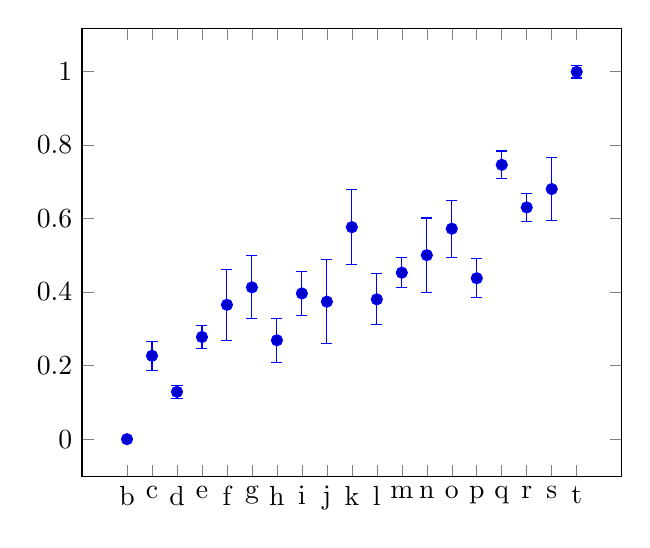
\begin{tikzpicture}
\begin{axis}[%
	%grid=both,%
	%xmajorgrids,%
	xtick={1,2,3,4,5,6,7,8,9,10,11,12,13,14,15,16,17,18,19},%
	xticklabels={b,c,d,e,f,g,h,i,j,k,l,m,n,o,p,q,r,s,t},%
]
% Line plot
\addplot
	plot[ 	%smooth,
	   		only marks,
	      	error bars/.cd,
	      	y dir=both, y explicit %
		]
	coordinates{
	(1,0) 			+- (0,0)
	(2,0.226697)	+- (0,0.0389)
	(3,0.128649)	+- (0,0.0174)
	(4,0.277819)	+- (0,0.0316)
	(5,0.365309) 	+- (0,0.0960)
	(6,0.412726)	+- (0,0.0856)
	(7,0.268849) 	+- (0,0.0598)
	(8,0.396237)	+- (0,0.0589)
	(9,0.373823)	+- (0,0.1148)
	(10,0.576375)	+- (0,0.1020)
	(11,0.380172) 	+- (0,0.0696)
	(12,0.452672)	+- (0,0.0404)
	(13,0.500303)	+- (0,0.1010)
	(14,0.572158)	+- (0,0.0778)
	(15,0.437586)	+- (0,0.0524)
	(16,0.745885)	+- (0,0.0376)
	(17,0.630023)	+- (0,0.0386)
	(18,0.679989)	+- (0,0.0852)
	(19,0.998734)	+- (0,0.0169)
};

\end{axis}
\end{tikzpicture}


% plot erstellt mit MATLAB-File p:\doc\MATLAB\WFS-CompareDMPs\wfs_Compare2008c.m (FromToTo = 1:5:1024)
% und matlab2tikz

%[ 1:19;std(NormCumulativeError);mean(NormCumulativeError)]
%
%ans =
%
%  Columns 1 through 12
%
%    1.0000    2.0000    3.0000    4.0000    5.0000    6.0000    7.0000    8.0000    9.0000   10.0000   11.0000   12.0000
%         0    0.0389    0.0174    0.0316    0.0960    0.0856    0.0598    0.0589    0.1148    0.1020    0.0696    0.0404
%         0    0.2267    0.1286    0.2778    0.3653    0.4127    0.2688    0.3962    0.3738    0.5764    0.3802    0.4527
%
%  Columns 13 through 19
%
%   13.0000   14.0000   15.0000   16.0000   17.0000   18.0000   19.0000
%    0.1010    0.0778    0.0524    0.0376    0.0386    0.0852    0.0169
%    0.5003    0.5722    0.4376    0.7459    0.6300    0.6800    0.9987          	
         	
%
%\end{preview}
%\end{document}%
		\label{fig:NormalizedErrorPlot}%
	\end{figure}%
\else
	\begin{figure}[htp]
		\centering
		%\documentclass{article}
%\usepackage{tikz,pgfplots}
%\usepackage[pdftex,active,tightpage]{preview}
%\begin{document}
%\begin{preview}

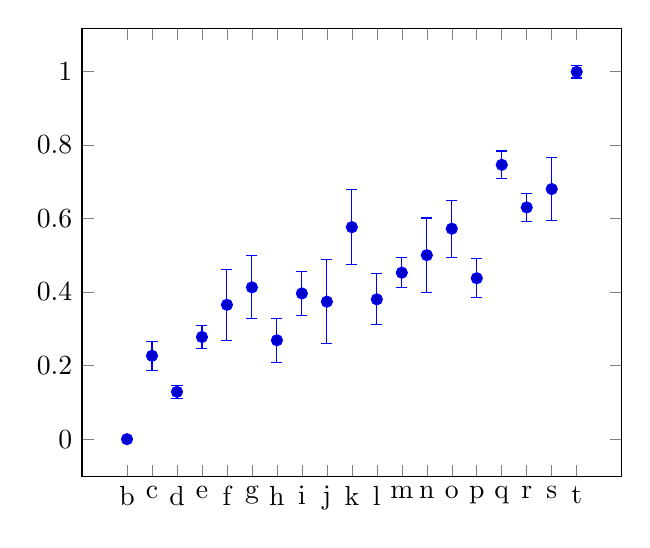
\begin{tikzpicture}
\begin{axis}[%
	%grid=both,%
	%xmajorgrids,%
	xtick={1,2,3,4,5,6,7,8,9,10,11,12,13,14,15,16,17,18,19},%
	xticklabels={b,c,d,e,f,g,h,i,j,k,l,m,n,o,p,q,r,s,t},%
]
% Line plot
\addplot
	plot[ 	%smooth,
	   		only marks,
	      	error bars/.cd,
	      	y dir=both, y explicit %
		]
	coordinates{
	(1,0) 			+- (0,0)
	(2,0.226697)	+- (0,0.0389)
	(3,0.128649)	+- (0,0.0174)
	(4,0.277819)	+- (0,0.0316)
	(5,0.365309) 	+- (0,0.0960)
	(6,0.412726)	+- (0,0.0856)
	(7,0.268849) 	+- (0,0.0598)
	(8,0.396237)	+- (0,0.0589)
	(9,0.373823)	+- (0,0.1148)
	(10,0.576375)	+- (0,0.1020)
	(11,0.380172) 	+- (0,0.0696)
	(12,0.452672)	+- (0,0.0404)
	(13,0.500303)	+- (0,0.1010)
	(14,0.572158)	+- (0,0.0778)
	(15,0.437586)	+- (0,0.0524)
	(16,0.745885)	+- (0,0.0376)
	(17,0.630023)	+- (0,0.0386)
	(18,0.679989)	+- (0,0.0852)
	(19,0.998734)	+- (0,0.0169)
};

\end{axis}
\end{tikzpicture}


% plot erstellt mit MATLAB-File p:\doc\MATLAB\WFS-CompareDMPs\wfs_Compare2008c.m (FromToTo = 1:5:1024)
% und matlab2tikz

%[ 1:19;std(NormCumulativeError);mean(NormCumulativeError)]
%
%ans =
%
%  Columns 1 through 12
%
%    1.0000    2.0000    3.0000    4.0000    5.0000    6.0000    7.0000    8.0000    9.0000   10.0000   11.0000   12.0000
%         0    0.0389    0.0174    0.0316    0.0960    0.0856    0.0598    0.0589    0.1148    0.1020    0.0696    0.0404
%         0    0.2267    0.1286    0.2778    0.3653    0.4127    0.2688    0.3962    0.3738    0.5764    0.3802    0.4527
%
%  Columns 13 through 19
%
%   13.0000   14.0000   15.0000   16.0000   17.0000   18.0000   19.0000
%    0.1010    0.0778    0.0524    0.0376    0.0386    0.0852    0.0169
%    0.5003    0.5722    0.4376    0.7459    0.6300    0.6800    0.9987          	
         	
%
%\end{preview}
%\end{document}
		\caption{Plot of normalized difference Value ($E_{norm}$, blue diamonds) for the 19 scanned protocols overlaid over Quality-plot (red dots) obtained from the simulation. The normalized Error has been calculated using the difference image of each protocol $i$ with protocol B. The error bars for each protocol show the standard deviation of the error which was calculated for 205 of the 1024 slices for each protocol. Note that the scale of the error been normalized to 20--\SI{100}{\percent}, so that both the quality from the simulation and the error are directly comparable. The abscissa shows the scanning time in percentage of time used for the gold standard scan. The protocols would be shown are in decreasing order from T--B for increasing percentage.}%
		\label{fig:NormalizedErrorPlot}
	\end{figure}
\fi

\subsubsection{Three dimensional visualization of different protocols}%
\label{subsec:comparison}%
The tomograms of the different protocols have been three dimensionally visualized and analyzed using MeVisLab (Version 1.6.1 (2008-09-21 Release), MeVis Medical Solutions AG, Bremen, Germany). Airway segments have been extracted using a threshold interval based region growing algorithm. A seed point for the region growing algorithm has been manually defined in the most proximal slice for each independent airway segment. The coordinates of the seed points have been kept constant for protocol B--T, allowing direct comparison of the airway segment reconstructions of the different protocols. Airway segments extracted for protocol B and T are shown in figure~\ref{fig:BvsT}.

The data shown in figure~\ref{fig:BvsT} represent two extremes of the 19 protocols used. Protocol B corresponds to a slightly oversampled gold standard scan, obtained with in total 15732 projections recorded in 65 minutes. Protocol T has been obtained in just 12 minutes, with in total 2185 projections. The tomographic dataset from protocol B has been reconstructed from 5244 merged projection images, the dataset from protocol T has been reconstructed using only 874 merged projections. Even if we scanned protocol T while violating the sampling theorem and with a total scanning time reduced by \SI{13.75}{\percent}, both samples still appear to be identical in the low-resolution three dimensional visualization as shown in figure~\ref{fig:BvsT}a) and b), except for small differences at the most lateral parts of the sample (yellow segment).

The artifacts introduced through the reduction in scanning time only become apparent at higher magnification. The blue cube inside the green airway segments in figures~\ref{fig:BvsT}a) and \ref{fig:BvsT}b) are shown as isosurface visualizations of the lung tissue (which exactly corresponds to the negative of the extracted airway segment) in figures~\ref{fig:BvsT}c) and \ref{fig:BvsT}d). Both regions of interest show a cube with a side length of \SI{190}{\micro\meter}. We observe that the isosurface of the ROI of protocol T shown in figure~\ref{fig:BvsT}d) appears rougher than the isosurface of protocol B shown in figure~\ref{fig:BvsT}c). This roughness is introduced through wave-like artifacts visible in the original slice of the dataset of protocol T (not shown\todo{since ``old'' figure 11 had been deleted\ldots}) which arise through the breaching of the sampling theorem, since we have only acquired 874 projections for the two ring-scans (2185 projections in total for protocol T) instead of the 5139 projections ($(3072-200)\frac{\pi}{2}$) which would be necessary to satisfy the sampling theorem. But even with this strong undersampling a segmentation, three dimensional reconstruction and visualization of the sample is still possible. Thus, if the user desired to gain a quick overview over his sample, e.g.\ to quickly assess the integrity of multiple samples over a short time, such a time-saving protocol could be used.

\ifiucr%%% iucr %%%
	%\onecolumn%
	\begin{figure}%
		\centering%
		\caption{Comparison of three-dimensional visualizations of protocols B and T. a): Three independent airway segments (green, red, yellow) of Protocol B have been extracted using a region growing algorithm. b): Same for protocol T. A cubical region of interest (ROI, blue) with a side length of 128 pixels (corresponding to \SI{190}{\micro\meter}) is marked inside the leftmost segment for both protocols. c): Detailed view of isosurfaces of the lung tissue inside the ROIs shown for protocol B. d): Same for protocol T. Note the artifacts in the isosurface in subfigure d).}%
		\renewcommand{\imsize}{.5\linewidth}%
		\pgfmathsetlength{\imagewidth}{\imsize}%
		\pgfmathsetlength{\imagescale}{\imagewidth/1397}%
		\def\x{100}%
		\def\y{150}%
		\begin{tikzpicture}[x=\imagescale,y=-\imagescale]%
			\node[anchor=north west,inner sep=0pt,outer sep=0pt] at (0,0)%
				{\includegraphics[width=\imagewidth]{img/comparisonBvsT/overview-b}};%
			% 1391px = 4.0138mm > 100px = 288um > 173px = 500um
%			\draw[|-|,thick] (6,774) -- (1395,839) node [sloped,midway,above] {\SI{4.0138}{\milli\meter}};%
			\draw[|-|,thick] (\x,\y) -- (\x+173,\y) node [midway,above] {\SI{500}{\micro\meter}};%
			\node [anchor=south west] at (0,899) {(a)};%
		\end{tikzpicture}%
		\begin{tikzpicture}[x=\imagescale,y=-\imagescale]%
			\node[anchor=north west,inner sep=0pt,outer sep=0pt] at (0,0)%
				{\includegraphics[width=\imagewidth]{img/comparisonBvsT/overview-t}};%
			% 1391px = 4.0138mm > 100px = 288um > 173px = 500um
%			\draw[|-|,thick] (6,774) -- (1395,839) node [sloped,midway,above] {\SI{4.0138}{\milli\meter}};%
			\draw[|-|,thick] (\x,\y) -- (\x+173,\y) node [midway,above] {\SI{500}{\micro\meter}};%
			\node [anchor=south west] at (0,899) {(b)};%
		\end{tikzpicture}%
		\\%
		\pgfmathsetlength{\imagescale}{\imagewidth/806}%
		\def\x{345}%
		\def\y{780}%
		\begin{tikzpicture}[x=\imagescale,y=-\imagescale]%
			\node[anchor=north west,inner sep=0pt,outer sep=0pt] at (0,0)%
				{\includegraphics[width=\imagewidth]{img/comparisonBvsT/roi-b-nomedian}};%
			% 746px = 0.18944mm > 100px = 25um > 196.9px = 50um
%			\draw[|-|,thick] (27,270) -- (773,272) node [sloped,midway,above] {\SI{189.44}{\micro\meter}};%
			\draw[|-|,thick] (\x,\y) -- (\x+196.9,\y) node [midway,above] {\SI{50}{\micro\meter}};%
			\node [anchor=south west] at (0,802) {(c)};%
		\end{tikzpicture}%
		\begin{tikzpicture}[x=\imagescale,y=-\imagescale]%
			\node[anchor=north west,inner sep=0pt,outer sep=0pt] at (0,0)%
				{\includegraphics[width=\imagewidth]{img/comparisonBvsT/roi-t-nomedian}};%
			% 744px = 0.18944mm > 100px = 25um > 196.5px = 50um
%			\draw[|-|,thick] (27,311) -- (771,311) node [sloped,midway,above] {\SI{189.44}{\micro\meter}};%
			\draw[|-|,thick] (\x,\y) -- (\x+196.5,\y) node [midway,above] {\SI{50}{\micro\meter}};%
			\node [anchor=south west] at (0,802) {(d)};%
		\end{tikzpicture}%
		\label{fig:BvsT}%
	\end{figure}%
\else
	\begin{figure}[htp]
		\renewcommand{\imsize}{.5\linewidth}
		\centering
		\pgfmathsetlength{\imagewidth}{\imsize}
		\pgfmathsetlength{\imagescale}{\imagewidth/1397} % pixel width of imagefile used
		\def\x{100}
		\def\y{150}
		\subfloat[Overview of protocol B]{%
			\begin{tikzpicture}[x=\imagescale,y=-\imagescale]
				\node[anchor=north west,inner sep=0pt,outer sep=0pt] at (0,0)
					{\includegraphics[width=\imagewidth]{img/comparisonBvsT/overview-b}};
				% 1391px = 4.0138mm > 100px = 288um > 173px = 500um
%				\draw[|-|,thick] (6,774) -- (1395,839) node [sloped,midway,above] {\SI{4.0138}{\milli\meter}};
				\draw[|-|,thick] (\x,\y) -- (\x+173,\y) node [midway,above] {\SI{500}{\micro\meter}};
			\end{tikzpicture}%
			}%
		\subfloat[Overview of protocol T]{%
			\begin{tikzpicture}[x=\imagescale,y=-\imagescale]
				\node[anchor=north west,inner sep=0pt,outer sep=0pt] at (0,0)
					{\includegraphics[width=\imagewidth]{img/comparisonBvsT/overview-t}};
				% 1391px = 4.0138mm > 100px = 288um > 173px = 500um
%				\draw[|-|,thick] (6,774) -- (1395,839) node [sloped,midway,above] {\SI{4.0138}{\milli\meter}};
				\draw[|-|,thick] (\x,\y) -- (\x+173,\y) node [midway,above] {\SI{500}{\micro\meter}};
			\end{tikzpicture}%
			}\\%
		\pgfmathsetlength{\imagescale}{\imagewidth/806} % pixel width of imagefile used
		\def\x{345}
		\def\y{780}
		\subfloat[ROI inside green segment for protocol B]{%
			\label{subfig:DetailROIB}%
			\begin{tikzpicture}[x=\imagescale,y=-\imagescale]
				\node[anchor=north west,inner sep=0pt,outer sep=0pt] at (0,0)
					{\includegraphics[width=\imagewidth]{img/comparisonBvsT/roi-b-nomedian}};
				% 746px = 0.18944mm > 100px = 25um > 196.9px = 50um
%				\draw[|-|,thick] (27,270) -- (773,272) node [sloped,midway,above] {\SI{189.44}{\micro\meter}};
				\draw[|-|,thick] (\x,\y) -- (\x+196.9,\y) node [midway,above] {\SI{50}{\micro\meter}};
			\end{tikzpicture}%
			}%
		\subfloat[ROI inside green segment for protocol T]{%
			\label{subfig:DetailROIT}%
			\begin{tikzpicture}[x=\imagescale,y=-\imagescale]
				\node[anchor=north west,inner sep=0pt,outer sep=0pt] at (0,0)
					{\includegraphics[width=\imagewidth]{img/comparisonBvsT/roi-t-nomedian}};
				% 744px = 0.18944mm > 100px = 25um > 196.5px = 50um
%				\draw[|-|,thick] (27,311) -- (771,311) node [sloped,midway,above] {\SI{189.44}{\micro\meter}};
				\draw[|-|,thick] (\x,\y) -- (\x+196.5,\y) node [midway,above] {\SI{50}{\micro\meter}};
			\end{tikzpicture}%
			}%
		\caption{Comparison of three-dimensional visualizations of protocols B and T. Top: Three independent airway segments (green, red, yellow) have been extracted using a region growing algorithm. A cubical region of interest (ROI, blue) with a side length of 128 pixels (corresponding to \SI{190}{\micro\meter}) is marked inside the leftmost segment for both protocols. Bottom: Detailed view of isosurfaces of the lung tissue inside the ROIs shown above. Note the artifacts in the reconstructions for protocol T in subfigure~\subref{subfig:DetailROIT}.}%
		\label{fig:BvsT}%
	\end{figure}
\fi

The field of view can be increased even further; we also scanned and reconstructed a rat lung sample with 5 scanning positions, resulting in a five-fold (4.74$\times$) increase in available field of view from 1024$\times$1024 pixels to 4850$\times$4850 pixels (data not shown). We have been able to reconstruct a sample with size of approximately 0.82$\times$7.18$\times$\SI{1.52}{\milli\meter} at a voxel side length of \SI{1.48}{\micro\meter}.